\documentclass[11pt]{article}
\usepackage{graphicx}
\DeclareGraphicsRule{.tiff}{png}{.png}{`convert #1 `dirname #1`/`basename #1 .tiff`.png}

\usepackage{amsmath,amssymb}
\usepackage{times}
\usepackage{epstopdf}
\usepackage[ligature,reserved]{semantic}
\usepackage[center,tight]{subfigure}

\textwidth = 6.5 in
\textheight = 9 in
\oddsidemargin = 0.0 in
\evensidemargin = 0.0 in
\topmargin = 0.0 in
\headheight = 0.0 in
\headsep = 0.0 in
\parskip = 0.2in
\parindent = 0.0in

\newtheorem{theorem}{Theorem}
\newtheorem{corollary}[theorem]{Corollary}
\newtheorem{definition}{Definition}

\title{Disproof in Jape (a short how-to note)}
\author{Richard Bornat (richard@bornat.me.uk)}

\mathlig{->}{\rightarrow}
\mathlig{|=}{\vDash}
\mathlig{!}{\neg}

\reservestyle{\word}{\operatorname}
\word{actual}

\reservestyle{\var}{\mathit}
\var{j1,j2}

\begin{document}
\maketitle

The \texttt{examples/natural\_deduction/I2L.jt} encoding of natural deduction in Jape allows for \emph{disproof} as well as proof. It allows you to make Kripke diagrams which Jape will check to see if they are examples or counter-examples (or neither) against a sequent which you choose.

If you have no notion what a Kripke diagram is, then maybe you can find out by playing, or maybe you will have to wait for my book (which will come out, so long as I deliver it to OUP in time!). This note is just about the mechanics, and what Jape can show you.

This note shows coloured diagrams, and may not make sense if printed in shades of grey.

\section{Basics}

At any point during a proof attempt you can invoke `Disprove' from the Edit menu.\footnote{There isn't a Disprove button on the Conjectures menus. Perhaps there should be! At present you have to hit Prove to start a prove attempt and then choose Disprove.} Jape splits the window and shows you a diagram with a single empty world and, by default, the proof-attempt sequent (see below for how to get a different sequent).

\begin{figure}
\begin{center}
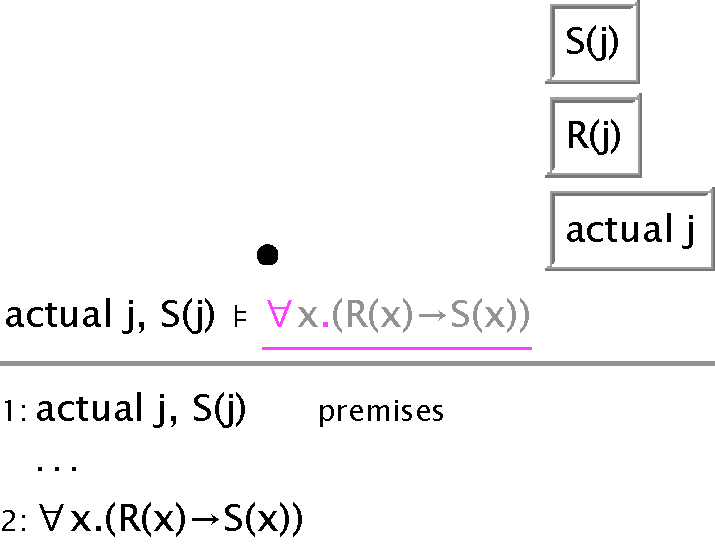
\includegraphics[scale=0.6]{pics/firstexample.tiff}
\caption{The start of a disproof attempt}
\label{fig:firstexample}
\end{center}
\end{figure}
Figure \ref{fig:firstexample} shows an example of what you see. The main things to notice are
\begin{itemize}
\item the single world is ringed in red;
\item some of the names and connectives in the sequent are violet, some are grey, and some are black;
\item some of the formulae are underlined and some are not;
\item the sequent uses the semantic turnstile $|=$; 
\item there's a little green waste bin on the right;
\item above the waste bin there are some tiles, each containing an atomic formula.
\end{itemize}
Your window may not look exactly like figure \ref{fig:firstexample}, but it will have the same parts. Other illustrations in this document show the important bits of the proof and/or disproof sections of the window, without the waste bin and the scroll bars and stuff.

\subsection{Alternative sequents}

If, during a proof attempt, you select a conclusion (or, if Jape doesn't want to let you do that, the reason next to the conclusion) and then hit Edit:Disprove, Jape will use the disproof sequent consisting of the conclusion formula and all the lines above it as hypothesis formulae. If you select some of the hypothesis lines, you can choose the collection of hypothesis formulae that appear.

You can choose a new disproof sequent at any time, even in the middle of a disproof attempt.

If you want to set up an entirely new challenge, enter it into one of the conjectures panels (New button), hit Prove and then Edit:Disprove in the proof window.

\subsection{Selecting a situation}

\begin{figure}
\centering
\parbox{200pt}{\centering
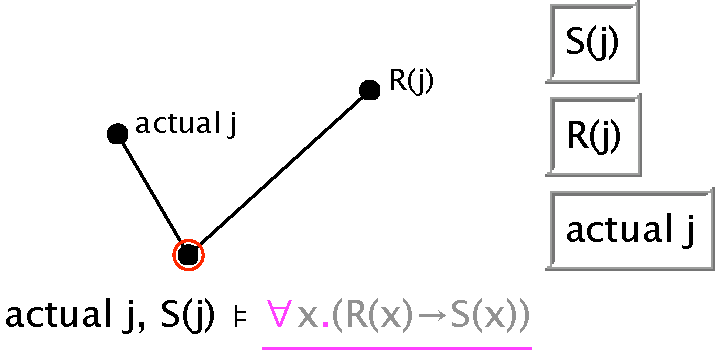
\includegraphics[scale=0.6]{pics/firstmultiworld}
\caption{A multi-world situation}
\label{fig:firstmultiworld}
}
\qquad
\parbox{200pt}{\centering
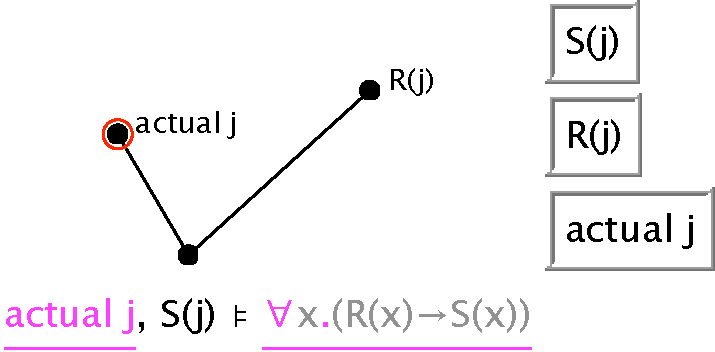
\includegraphics[scale=0.6]{pics/parvainmultum}
\caption{A single-world situation}
\label{fig:parvainmultum}
}
\end{figure}
By selecting a world you define a `situation' comprising the world and all the worlds you can reach above it. The root world of the situation is ringed in red to show that it is selected. There is always exactly one selected world, and therefore exactly one situation. Figure \ref{fig:firstmultiworld} shows a situation with more than one world; figure \ref{fig:parvainmultum} shows a single-world situation inside a multi-world diagram.

\subsection{What's forced ? -- colouring, greying, underlining}

Jape evaluates all the formulae and sub-formulae in the sequent and colours them. 
\begin{itemize}
\item The default colour is black, and it means \emph{not forced}.
\item If a (sub-)formula's value is never called on -- usually this is true of quantified predicates, for example -- then it's grey, meaning \emph{strictly irrrelevant}.
\item An atomic (sub-)formula which is \emph{forced} is coloured violet (this covers atoms like $E$, atomic predicates like $S(j)$ and individuals like $\<actual> k$).
\item When a non-atomic (sub-)formula is forced, its connective is coloured violet. 
\item When an entire sequent hypothesis or conclusion is forced, it is underlined in violet.
\end{itemize}
So when all the premises are underlined and the conclusion is not, you have a counter-example; when everything is underlined you have an example; otherwise you have nothing in particular.

\begin{figure}
\centering
\parbox{150pt}{\centering
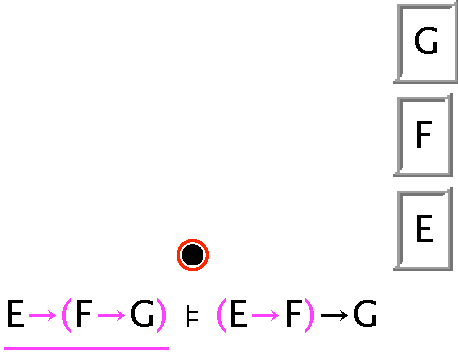
\includegraphics[scale=0.6]{pics/firstcounterexample}
\caption{A simple counter-example}
\label{fig:firstcounterexample}
}
\qquad
\parbox{250pt}{\centering
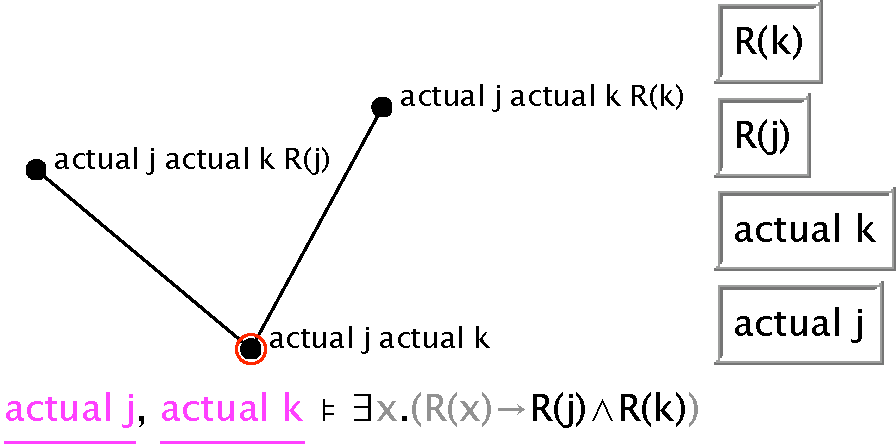
\includegraphics[scale=0.6]{pics/elaboratecounterexample}
\caption{An elaborate counter-example}
\label{fig:elaboratecounterexample}
}
\end{figure}

Figure \ref{fig:firstcounterexample} shows a sample counter-example, and the colouring gives a hint of why that is: $E$ isn't forced anywhere, so the hypothesis implication is forced; and then, because $E->F$ is forced but $G$ isn't, the conclusion isn't forced. Figure \ref{fig:elaboratecounterexample} shows an elaborate counter-example, and the colouring isn't much help at all.\footnote{I have some ideas which might help in this case, but I haven't implemented them yet.}

Figure 1 is neither a counter-example nor an example. The hypotheses aren't forced because, as atomic formulae, they aren't present at the root world; the conclusion is forced because every individual in the situation (there aren't any ..) forces a version of $R(x)->S(x)$. Similar remarks apply to figures \ref{fig:firstmultiworld} and \ref{fig:parvainmultum}.

\section{Making diagrams}

To begin your disproof Jape presents you with the simplest diagram: the isolated empty world. You add parts of your diagram -- worlds, formulae and lines -- using drag-and-drop mouse gestures. You can delete the same components by dragging them to the waste bin. You can add tiles with double-clicks. You can Undo your actions to any degree that you like, and Redo likewise.\footnote{Undo and Redo apply to the last pane you clicked, either proof or disproof.} 

\subsection{Making new worlds}

By dragging on a world with the middle mouse button or by holding down the alt shift key while dragging with a single-button mouse, you drag a copy of the world with a line attaching it to the world it came from.

The new world stays where you put it. If it's above the world you dragged it from, they will be connected by a line. If it's level or below, then no line.

Jape preserves monotonicity, so the new world will contain all the formulae that the original world did.

\subsection{Dragging worlds}

You can drag worlds about the place to make your diagram look nicer. You use the left mouse button on a multibutton mouse. Jape will delete a line if you drag a world below its parent.

You can drag a world onto a line (which lights up to show you are over it) or another world (which lights up ditto) and Jape does the obvious thing, adding whatever formulae are necessary to whatever worlds in order to maintain monotonicity.

If you drag a world to the waste bin it's deleted, along with all the formulae attached to it and all the lines connected to it. The bin lights up when it will accept the world; it won't accept the currently-selected world.

\subsection{Making lines}

If you want to make a line between world A and world B, where A is below B, make-world-drag from A to B and drop the new world onto B. Jape makes the monotonicity adjustments. Dragging from B to A has some effect, but perhaps not a very useful effect (but there's always Undo!).

\subsection{Dragging lines}

You can drag lines and drop them onto worlds or into the waste bin, as you wish. Jape does the obvious thing in each case (if you can't guess what that is, just try it!).

\subsection{Dragging formulae}

You can drag a formula from a tile and drop it onto a world (the world lights up, of course, to show that it's eager to accept; worlds won't accept a second copy of a formula they already have). The formula isn't deleted from the tile.

You can drag a formula from one world onto another; it is added to the destination world (and not deleted from the source world).

Jape preserves monotonicity, so all worlds reachable from the destination world get a copy of the dropped formula as well.

If you let go of a formula when you aren't over a world that has lit up to accept it, it flies back to base.

If you drag a formula from a world to the waste bin it is deleted from that world (and then, to preserve monotonicity, from its parents and its grandparents and so on down).

\section{Making individuals and predicate instances}

If a sequent mentions an individual by including a hypothesis like $\<actual> j$, then there will be a tile for that individual (see figures \ref{fig:firstexample}, \ref{fig:firstmultiworld}, \ref{fig:parvainmultum} and \ref{fig:elaboratecounterexample}, for example). If there are quantifiers but no individuals you will get a free $\<actual> i$ tile.

If you need more individuals, double-click any individual tile. Jape uses a boring but obvious numbering algorithm to name the new individual -- $\<actual> j$, for example, generates first $\<actual> \<j1>$ then $\<actual> \<j2>$, and so on.

If you want to make a new predicate instance, double-click a predicate-instance tile. Jape looks through your tiles for unused individuals and uses them to give you a new one. For example if you have a tile showing $S(j)$ and individuals $\<actual> j$ and $\<actual> \<j1>$, then double-clicking $S(j)$ gets you $S(\<j1>)$, as you might expect. If there's more than one instance that could be made, Jape shows you the alternatives and asks you to choose. If you don't have enough individuals to make a new instance, it tells you so.

\begin{figure}
\centering
\parbox{150pt}{\centering
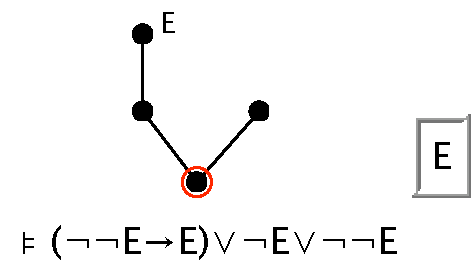
\includegraphics[scale=0.6]{pics/samuels0}
\caption{A counter-example}
\label{fig:samuels0}
}
\qquad
\parbox{150pt}{\centering
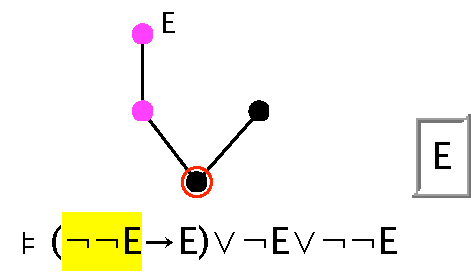
\includegraphics[scale=0.6]{pics/samuels1}
\caption{$!!E$ forced here}
\label{fig:samuels1}
}
\parbox{150pt}{\centering
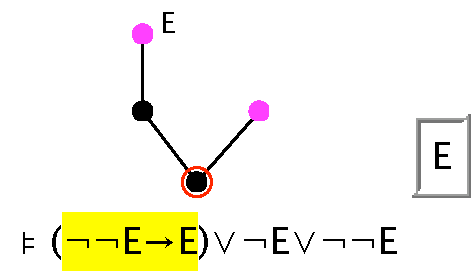
\includegraphics[scale=0.6]{pics/samuels2}
\caption{$!!E->E$ forced here}
\label{fig:samuels2}
}
\qquad
\parbox{150pt}{\centering
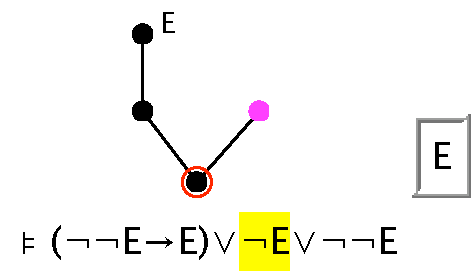
\includegraphics[scale=0.6]{pics/samuels3}
\caption{$!E$ forced here}
\label{fig:samuels3}
}
\parbox{150pt}{\centering
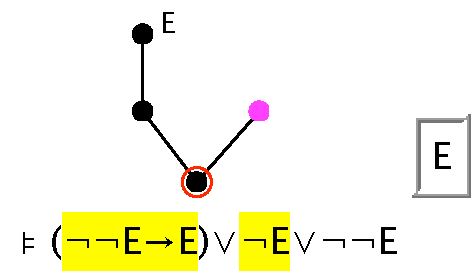
\includegraphics[scale=0.6]{pics/samuels4}
\caption{Multiple forcing}
\label{fig:samuels4}
}
\qquad
\parbox{150pt}{\centering
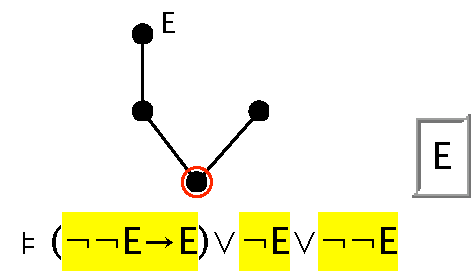
\includegraphics[scale=0.6]{pics/samuels5}
\caption{Too much forcing}
\label{fig:samuels5}
}
\end{figure}

\section{Exploring reasons}

The hardest thing to explain to a novice is \emph{why} a particular formula is forced in a particular situation. Figure \ref{fig:samuels0} shows a particularly ludicrous formula and its counter-example, which really needs explanation.

Jape provides some mechanisms which can be some help (in versions v6.2.a1.2 and later).

First, the colouring of atomic (sub-)formulae and connectives can help. But with the negative connectives -- $->$ and $!$ -- and with the quantifiers, we often need more help.

Second, Jape allows you to \emph{text-select} -- alt+press-and-drag, or middlebutton press-and-drag -- a subformula (or select a formula) in the sequent. It will then colour violet all the worlds which force the selected (sub)formula. For example, figure \ref{fig:samuels1} shows where $!!E$ is forced in our difficult example. Figures \ref{fig:samuels2} and \ref{fig:samuels3} show information about some other subformulae.

\subsection{Multiple selections}

If you choose more than one formula, as in figure \ref{fig:samuels4}, for example, Jape shows you where they are \emph{all} forced. If you choose too many formulae, as in figure \ref{fig:samuels5}, you may find that there is no subsituation which forces them all. But that's explanation too!

\begin{figure}
\centering
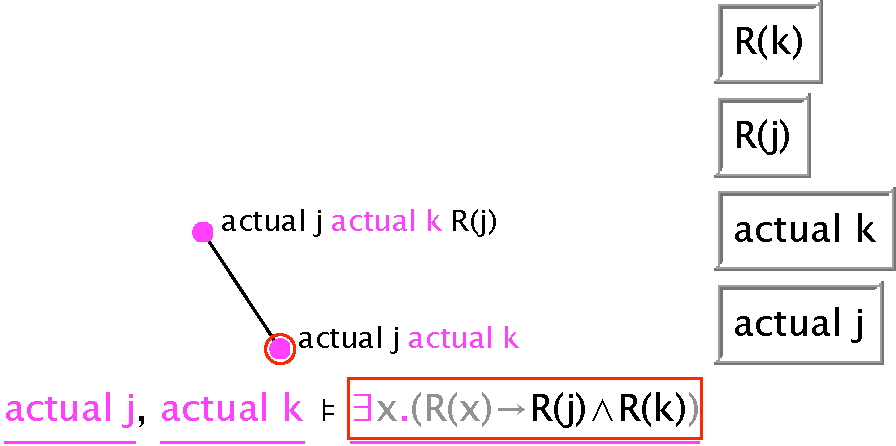
\includegraphics[scale=0.6]{pics/quantifiers1}
\caption{Support for a quantifier}
\label{fig:quantifiers1}
\end{figure}

\subsection{Quantifier reasons}

The world-colouring trick works well, but it isn't enough when you are dealing with quantifiers. You would like to know which individual formulae in the tree support the quantifier, and which do not. Jape can do that (in versions v6.2.a1.3 and later) by colouring individuals in the tree. In figure \ref{fig:quantifiers1}, for example, worlds which force the selected quantifier are violet; individuals which support the quantifier (those which generate a forced formula if you instantiate the quantified formula with them) are violet too. You can work out that $R(k)->R(j)@R(j)$ at each of the worlds of figure \ref{fig:quantifiers1}.

This isn't enough in general. You would like to be able to see those instantiations and play with them -- see why they are forced (or not, as the case may be). I think I can see how to build a Jape which could do that, but it doesn't do it at present.

\section*{How to complain}

If Jape doesn't work for you, it doesn't work. It's best to send your tales of woe to bugs@jape.org.uk. One day there'll be a mechanism to let you see other people's messages, but at the moment it's a private conversation.

\end{document} 